% =====================================================================
\chapter{Las aplicaciones}\label{cap:aplicaciones}

\section{Panorama}
\begin{center}\small
\begin{tabularx}{\linewidth}{>{\raggedright}p{3.6cm} >{\raggedright}p{3.8cm} >{\raggedright\arraybackslash}X}
\toprule
\textbf{Aplicación} & \textbf{Dónde corre} & \textbf{Para qué}\\
\midrule
STEP 7-Micro/WIN & máquina virtual Windows XP (VirtualBox) en la PC de Linux; o Windows directo & editar, compilar y cargar los programas del PLC; el USB del cable se pasa a la VM desde \emph{Dispositivos $\rightarrow$ USB}\\
App del gemelo (\codigo{app/}) & PC del laboratorio, Linux o Windows, Python 3 & conectar con el PLC, ver y mandar el brazo; menú de tres modos; acceso por red\\
Página publicada & internet (GitHub Pages y Cloudflare Pages) & documentación del proyecto, simulación del brazo, catálogo de archivos\\
Scripts de modelado & cualquier PC (Node.js, Python, MATLAB) & cinemática, gráficas, modelo 3D\\
\bottomrule
\end{tabularx}
\end{center}

\section{Arquitectura de tres capas}
La guía 1 pide pensar el sistema en tres capas. Así quedaron:
\begin{figure}[H]
\centering
\begin{tikzpicture}[node distance=5mm and 10mm, capa/.style={draw, rounded corners=3pt, fill=gris!60, minimum width=4.2cm, minimum height=48mm, align=center, font=\small\bfseries, anchor=north}]
\node[capa] (c1) at (0,0) {};
\node[capa] (c2) at (5,0) {};
\node[capa] (c3) at (10,0) {};
\node[font=\small\bfseries, below=1mm of c1.north] {Campo y control};
\node[font=\small\bfseries, below=1mm of c2.north] {Aplicación (middleware)};
\node[font=\small\bfseries, below=1mm of c3.north] {Datos y presentación};
\node[cajab, text width=3.4cm, font=\scriptsize] at (0,-1.6) {sensores, panel, drivers, motores};
\node[cajan, text width=3.4cm, font=\scriptsize] at (0,-3.4) {PLC S7-200 con \codigo{brazo\_gemelo}: cuenta, protege, ejecuta};
\node[cajab, text width=3.4cm, font=\scriptsize] at (5,-1.6) {\codigo{ppi.py} + \codigo{serie.py}: lee y escribe el PLC};
\node[cajan, text width=3.4cm, font=\scriptsize] at (5,-3.4) {\codigo{brazo.py} + \codigo{gemelo\_brazo.py}: estado, órdenes, usuarios, API};
\node[cajab, text width=3.4cm, font=\scriptsize] at (10,-1.6) {página del gemelo (3D) en la PC y en celulares};
\node[cajab, text width=3.4cm, font=\scriptsize, dashed] at (10,-3.4) {PostgreSQL (capítulo \ref{cap:datos}): telemetría e historial};
\draw[dflecha] (c1.east |- 0,-2.4) -- node[above, etiq]{PPI} (c2.west |- 0,-2.4);
\draw[dflecha] (c2.east |- 0,-2.4) -- node[above, etiq]{HTTP/JSON} (c3.west |- 0,-2.4);
\end{tikzpicture}
\caption{Arquitectura de tres capas del gemelo. La base de datos (línea punteada) está diseñada pero no conectada.}
\end{figure}

\section{La app del gemelo}
\subsection{Módulos}
\begin{center}\small
\begin{tabularx}{\linewidth}{>{\raggedright}p{3.6cm} >{\raggedright\arraybackslash}X}
\toprule
\textbf{Archivo} & \textbf{Responsabilidad}\\
\midrule
\codigo{gemelo\_brazo.py} & programa principal: menú de modos, cambio de modo en caliente, servidor local (127.0.0.1:8050) y de red (0.0.0.0:8443 con HTTPS), sesiones, filtros de órdenes, administración de usuarios\\
\codigo{brazo.py} & clase \codigo{Brazo} (bucle de lectura, mando, registro), \emph{perfiles} por programa del PLC, estimador, PLC simulado\\
\codigo{ppi.py} & cliente PPI (capítulo \ref{cap:ppi})\\
\codigo{serie.py} & puerto serie: termios en Linux, API Win32 por \codigo{ctypes} en Windows; lista de puertos\\
\codigo{acceso.py}, \codigo{usuarios.py} & contraseñas PBKDF2-SHA256 con 200\,000 iteraciones y sal propia; sesiones de 8~h; bloqueo de 60~s tras 5 fallos\\
\codigo{certificado\_tls.py} & genera el certificado HTTPS autofirmado en Python puro (RSA 2048, SHA-256)\\
\codigo{ventana.py} & ventana propia: GTK + WebKit (Linux) o Edge en modo aplicación (Windows)\\
\codigo{probar\_plc.py} & diagnóstico de solo lectura\\
\codigo{menu.html}, \codigo{ui/} & interfaz: menú y página del gemelo (copia de \codigo{web/js} hecha por \codigo{empaquetar.py})\\
\bottomrule
\end{tabularx}
\end{center}

\subsection{Hilos de ejecución}
\begin{figure}[H]
\centering
\begin{tikzpicture}[node distance=4mm, hilo/.style={draw, rounded corners=2pt, fill=white, text width=3.3cm, align=center, font=\scriptsize, minimum height=12mm}]
\node[hilo, fill=naranja!12] (h1) {\textbf{bucle del Brazo}\\lee el PLC sin pausa (6/s), envía el latido, reconecta};
\node[hilo, right=of h1] (h2) {\textbf{servidor local}\\127.0.0.1:8050\\un hilo por petición};
\node[hilo, right=of h2] (h3) {\textbf{servidor de red}\\0.0.0.0:8443, HTTPS\\(solo en ese modo)};
\node[hilo, right=of h3] (h4) {\textbf{vigilancia}\\suelta el mando si la sesión venció};
\node[hilo, below=8mm of h2, fill=gris] (h5) {\textbf{ventana}\\GTK o Edge (hilo principal)};
\node[cajan, below=8mm of h1, text width=3.3cm, font=\scriptsize] (m) {estado en memoria\\(protegido con \codigo{Lock})};
\draw[flecha] (h1) -- (m); \draw[flecha] (m) -- (h2); \draw[flecha] (m.east) -- ++(0.4,0) |- (h3.south);
\end{tikzpicture}
\caption{Hilos de la app. Las páginas nunca esperan al PLC: leen el último estado guardado.}
\end{figure}

\subsection{Perfiles: la app se adapta al programa del PLC}
\begin{center}\small
\begin{tabularx}{\linewidth}{>{\raggedright}p{2cm} >{\raggedright}p{3.6cm} >{\raggedright}X >{\raggedright\arraybackslash}p{3.2cm}}
\toprule
\textbf{Perfil} & \textbf{Se reconoce por} & \textbf{Lee} & \textbf{Órdenes}\\
\midrule
gemelo & VB1141 = \codigo{16\#47} & 40 bytes desde VB1120: posición contada, estado, error, E/S & homing, mover, garra, detener, velocidad\\
cargado & VD340/VD344 = 30000/25000 & E/S, SMB66--85 (PTO), VB200, VB300 y VW320: estima la posición & iniciar, detener, emergencia, rearmar, garra\\
monitor & cualquier otro & E/S y PTO; estima la posición & ninguna\\
\bottomrule
\end{tabularx}
\end{center}

\begin{lstlisting}[style=py, caption={Lectura del estado con el perfil \emph{gemelo} (\texttt{brazo.py}, fragmento).}]
def leer(self):
    v = self.cli.leer('V', 1120, 40)                    # una sola petición PPI
    estado, ack, flags, err = v[0], v[1], v[2], v[3]
    nz, nx, ny = struct.unpack('>iii', v[4:16])         # posición contada (big-endian)
    ib0, ib1, qb0 = v[18], v[19], v[20]
    sz, sx, sy = struct.unpack('>iii', v[24:36])        # tramo en curso
    # ... mientras un tramo está en marcha, se interpola su avance con el tiempo y el ciclo,
    # porque el PLC suma el tramo a la posición recién al terminarlo
\end{lstlisting}

\subsection{El estimador (programa original)}\label{sec:estimador}
Con el programa original el PLC no cuenta la posición. La app la estima en cada lectura:
\begin{enumerate}
\item si un PTO está ocupado, suma $f\,\Delta t$ pulsos, con $f = 10^6/\text{ciclo}$ leído de SMW68/SMW78;
\item reparte: PTO0 $\to$ base; PTO1 $\to$ X si K1 está cerrado e Y si K2 lo está; el signo sale de la DIR;
\item los tramos largos (homing, secuencias) se ajustan al número exacto de pulsos al terminar;
\item el jog del panel se integra con un factor de trabajo (0,93, SUPUESTO) que se \emph{autocalibra} cuando un carro va de un final de carrera al otro;
\item los finales de carrera y el inductivo corrigen la estimación al activarse.
\end{enumerate}
Prueba automática (\codigo{pruebas\_estimador.py}, con el PLC simulado imitando al programa original): error máximo de 1,35~mm en X/Y.

\subsection{El PLC simulado}
\codigo{PLCSimulado} imita al programa \codigo{brazo\_gemelo} con la misma interfaz que el cliente PPI (\codigo{leer}, \codigo{escribir}): avanza los ejes a la frecuencia pedida, respeta finales de carrera, homing, tramo común/resto, errores y watchdog. Lo usan el modo \emph{Simulación} y las pruebas.

\subsection{Modos y menú}
\begin{figure}[H]
\centering
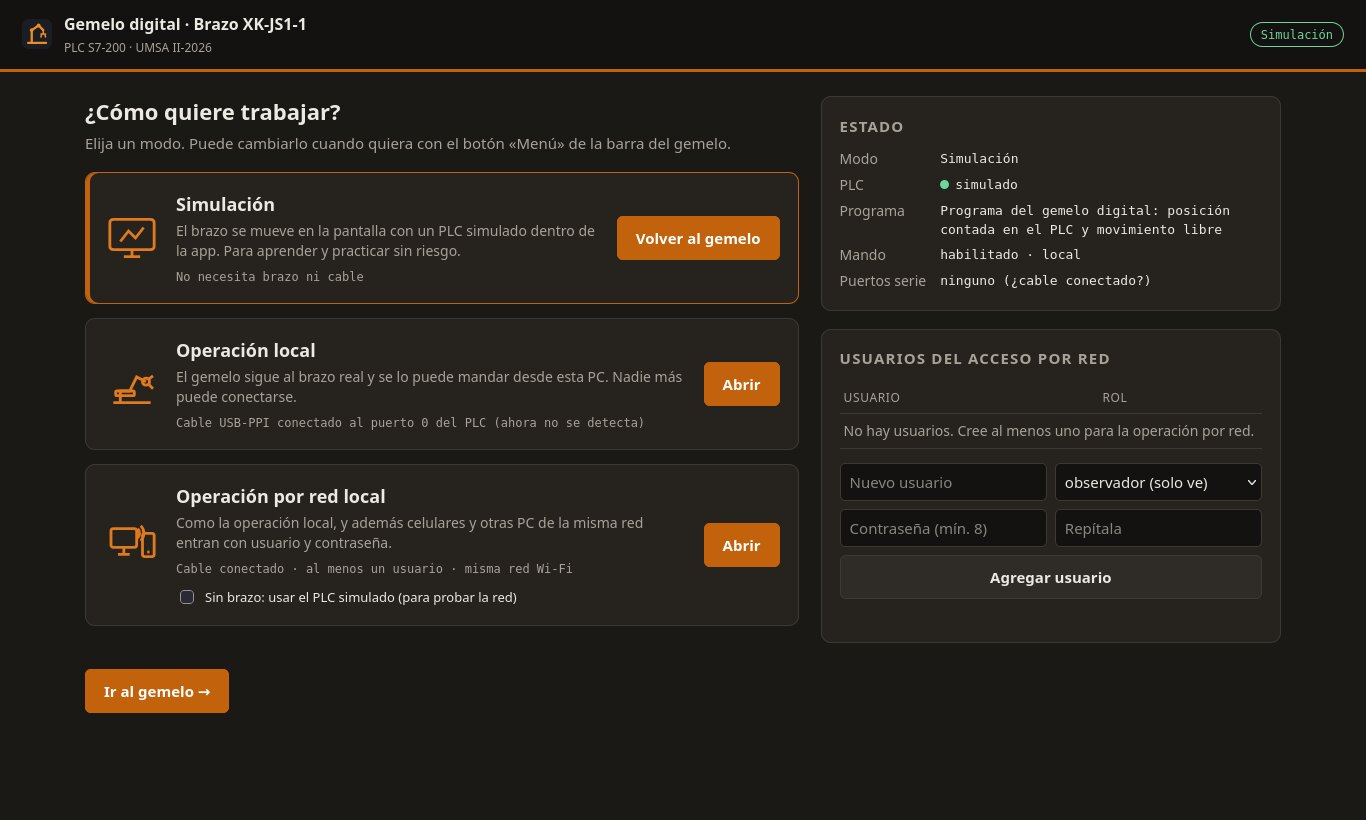
\includegraphics[width=0.85\linewidth]{menu_inicio.jpg}
\caption{Menú de la app.}
\end{figure}
\begin{lstlisting}[style=py, caption={Cambio de modo (\texttt{gemelo\_brazo.py}).}]
def aplicar_modo(modo, red_simulado=False):
    if modo == 'red' and not ACCESO.hay_usuarios():
        raise ValueError('para la operación por red cree antes al menos un usuario')
    simulado = modo == 'simulacion' or (modo == 'red' and red_simulado)
    with CAMBIO:
        if BRAZO is None or BRAZO.simulado != simulado:
            if BRAZO:
                BRAZO.cerrar()                  # detiene el brazo y suelta el puerto
            BRAZO = Brazo(Config.puerto, Config.direccion, simulado, REGISTRO)
        if modo == 'red':
            _activar_red()                      # servidor HTTPS en 0.0.0.0:8443
        else:
            _desactivar_red()
\end{lstlisting}

\subsection{API HTTP}
\begin{center}\small
\begin{longtable}{>{\ttfamily}p{4.6cm} >{\raggedright}p{2.6cm} >{\raggedright\arraybackslash}p{7.8cm}}
\toprule
\textbf{\rmfamily Ruta} & \textbf{Quién} & \textbf{Qué hace}\\
\midrule
\endhead
GET /api/estado & sesión & posición, E/S, mando, conexión (6 veces por segundo)\\
GET /api/info & sesión & programa reconocido, órdenes admitidas, transmisión\\
GET /api/sesion & sesión & usuario, rol, conectados\\
POST /api/mando & operador & tomar o soltar el mando\\
POST /api/orden/<nombre> & operador con mando & homing, mover, garra, detener, velocidad, \dots\\
POST /api/calibrar\_base & operador & calcula los pulsos por grado\\
GET /menu, GET /api/app & solo esta PC & menú y su estado\\
POST /api/app/modo & solo esta PC & cambiar de modo\\
POST /api/app/usuarios & solo esta PC & agregar, cambiar clave o rol, quitar\\
GET/POST /login, GET /salir & todos & ingreso y salida (acceso por red)\\
\bottomrule
\end{longtable}
\end{center}

\subsection{Seguridad y control de acceso por roles}\label{sec:acceso}
\begin{itemize}
\item \textbf{Dos puertas}: la local (127.0.0.1) no sale a la red y no pide contraseña; la de red (8443) exige HTTPS, usuario y rol.
\item \textbf{Roles} (RBAC): \emph{observador} solo lee; \emph{operador} puede tomar el mando. Un solo mando a la vez; cualquier operador puede dar paro.
\item \textbf{Filtros de cada orden}: sesión válida, origen de la propia página (contra sitios ajenos), rol, mando, selector en automático, homing previo; y luego los límites del PLC.
\item \textbf{Contraseñas}: PBKDF2-SHA256, 200\,000 iteraciones, sal aleatoria por usuario; \codigo{usuarios.json} no se sube al repositorio.
\item \textbf{Registro}: cada ingreso, orden aceptada u orden rechazada queda en \codigo{registro\_gemelo.log}.
\end{itemize}

\section{La página publicada}
\begin{figure}[H]
\centering
\begin{tikzpicture}[node distance=5mm and 9mm]
\node[cajab, text width=2.6cm] (push) {\codigo{git push}\\a \codigo{main}};
\node[caja, text width=3.2cm, right=of push, yshift=8mm] (gha) {GitHub Actions\\\codigo{pages.yml}:\\\codigo{build-catalog.js}};
\node[caja, text width=3.2cm, right=of push, yshift=-8mm] (cf) {Cloudflare Pages:\\\codigo{build-catalog.js}};
\node[cajan, text width=3.6cm, right=of gha] (ghp) {GitHub Pages};
\node[cajan, text width=3.6cm, right=of cf] (cfp) {\codigo{brazo-4gdl-gemelo-}\\\codigo{digital.pages.dev}};
\draw[flecha] (push) -- (gha); \draw[flecha] (push) -- (cf); \draw[flecha] (gha) -- (ghp); \draw[flecha] (cf) -- (cfp);
\end{tikzpicture}
\caption{Publicación automática de la página en cada \texttt{push} a \texttt{main}.}
\end{figure}
\codigo{scripts/build-catalog.js} recorre \codigo{global/} y \codigo{semestres/} y genera \codigo{web/data/catalogo.js}, el índice de documentos, programas y fotos que muestra la página. Los títulos y descripciones se corrigen en \codigo{config/archivos.json}. La sección \emph{Modelo 3D} de la página es la misma que usa la app (\codigo{web/js/modelo3d.js}, \codigo{cinematica.js}, \codigo{conexion-plc.js} y three.js 0.160).

\begin{figure}[H]
\centering
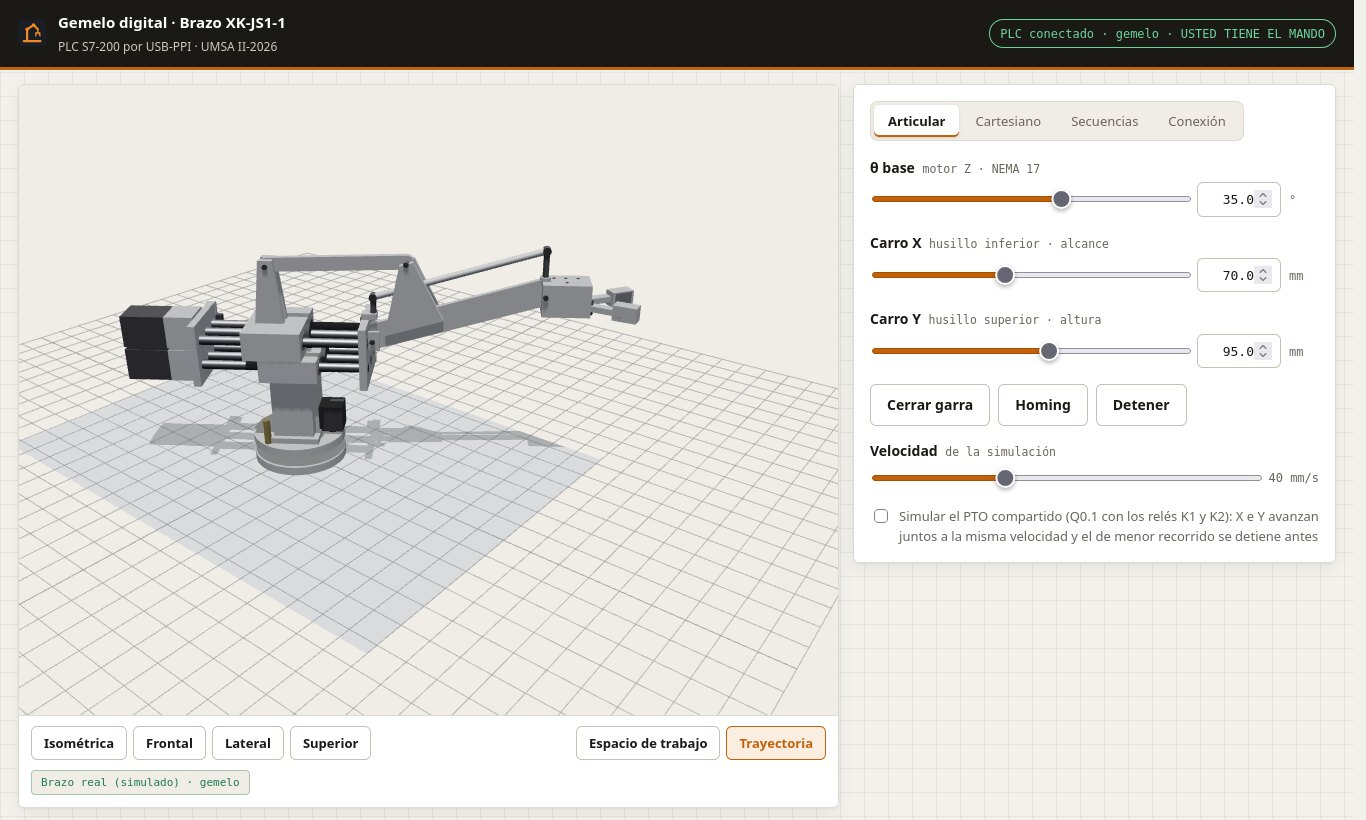
\includegraphics[width=0.85\linewidth]{local_articular.jpg}
\caption{Página del gemelo dentro de la app (modo simulación).}
\end{figure}
